\documentclass{article}
\usepackage[utf8]{inputenc}
\usepackage{xcolor}

\newcommand{\fixme}[1]{\textcolor{red}{#1}}

\title{3D Reconstruction \\ \small{Computer Vision 2}}

\author{Finde Xumara \\ ?????? \and Luka Stout \\ 10616713}

\begin{document}

\maketitle

%The report should be to the point, but complete. Based on the report we will grade your understanding, the final result and the correctness of your code (do not put large code listings! Only show the essential lines).
%The report is judged on your understanding. Do not ‘just’ do the assignments. Always give us your reasons why you did something. If possible, evaluate the effect of parameters, give insight, and explain the steps.

\section{Introduction}
\label{intro}
In this report wel will discuss the process we went through to make a 3D reconstruction from a set of photos. To do this we will use multiple techniques, including, keypoint extraction \cite{SIFT}, keypoint matching \cite{FLANN_based_matcher}, Structure from Motion \cite{SfM} and \fixme{Assignment4 technique?}.
In Section \ref{matching} we will discuss how we extracted featurepoints from an image. In Section \ref{structure} we will show how we used Structure from Motion to generate a 3D point cloud. In Section \fixme{The part about the last assignment}. Section \ref{experiments} will detail the results of the techniques used in this report.

\section{Keypoint extraction and matching}
\label{matching}
<<<<<<< HEAD
The first step in making a 3D reconstruction is to extract feature points from the two images.
Feature points are points of interest in an image and there are multiple ways of extracting them from an image.
A good feature points extracted from a descriptors should be repeatable, unique and consistent for all images;
occupies a relatively small area of the image (for robust to clutter and occlusion); and has a compact representation.
For example one could use dense sampling \cite{DSIFT} or random sampling,
however both these method did not prove to be useful when used in conjunction with the descriptors that we use for these keypoints.
In this report we will use the SIFT feature descriptors, introduced by Lowe\cite{SIFT} in 2004, as it has been the de facto representation method for feature points for the past years.

SIFT can robustly identify objects even among clutter and under partial occlusion, because it is invariant to uniform scaling, orientation, and partially invariant to illumination changes and affine distorting up to 60 degrees out of plane rotation.
To find keypoints SIFT uses Scale-space Extrema Detection.
It is a method to find points using the Differences of Gaussians (DoG) in a scale dependent way, to only find points that have the highest DoG in the area, which, after some refinement it can use as keypoints.
Around these keypoints a $16x16$ area is taken, which is then divided into $4x4$ subblocks.
Inside these subblocks a 8 bin orientation histogram is taken, so a 128 length feature vector is created as a representation of a keypoint.
Keypoints SIFT detect the unique corners in the image, therefore we need to have a source image with enough texture in order to have enough number of feature points.

We use a brute force matcher to match SIFT descriptors between images. 
For every keypoint in the first image we will find the keypoints with the smallest and the next-to-smallest euclidian distance in the second image. 
To filter out ambiguous matches we applied a ratio test. 
If the distance of the best match was bigger then a ratio of the second-to-best match then the keypoints were discarded.
By doing this ratio test reduction, we can remove keypoints that are not relevant for matching.

\begin{figure}[!ht]
	\centering
	\subfloat[Left bus image]{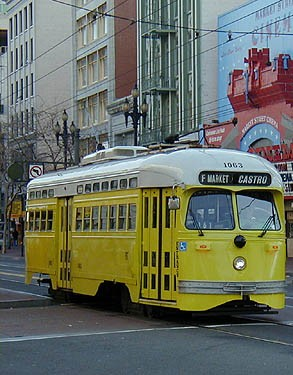
\includegraphics[width=.4\textwidth]{bus_left}} \quad
	\subfloat[Right bus image]{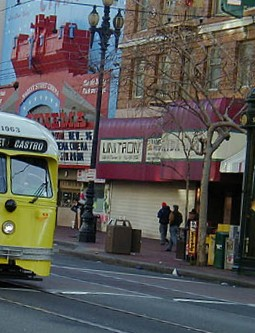
\includegraphics[width=.4\textwidth]{bus_right}}\\
	\subfloat[Matches between the images]{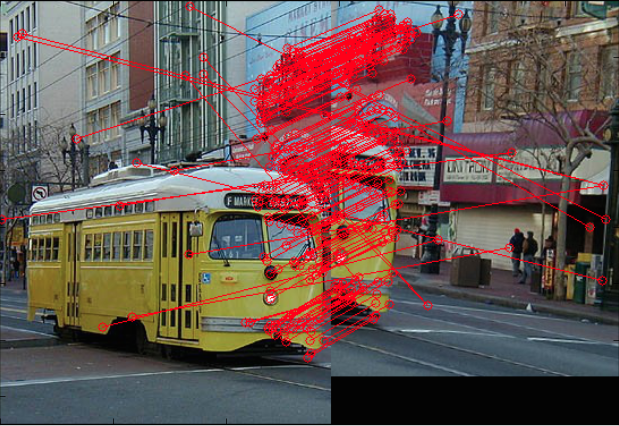
\includegraphics[width=.4\textwidth]{bus_matches}} \quad
	\subfloat[The two bus images stitched together]{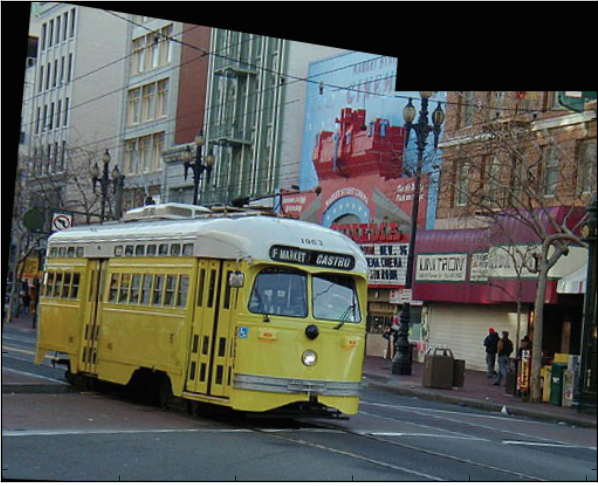
\includegraphics[width=.4\textwidth]{bus_stitched}}
	\caption{The red lines between the images are the matches that are found.}
	\label{fig:bus}
\end{figure}

After we have a good set of feature points representation, we can then estimate a homography matrix using RANSAC \cite{RANSAC}. 
In this report we implemented the improved version of RANSAC, namely Locally Optimized RANSAC (LO-RANSAC) \cite{LORANSAC}.
For the matching model, we used projection transformation matrix to make it robust to the images that were taken from different angles and distances.
We use this projection transformation because we assume that the camera point is not changed, therefore there is a homography between two views.

We found after some experiments that this value however does not work as well for teddy bear data (seen in Figure~\ref{fig:bear} set that we will try to reconstruct,
too many points get removed to still be able to reconstruct the teddy bear,
so we decided to have a ratio of $.75$ there.

\begin{figure}[ht]
	\centering
	\includegraphics[width=.45\textwidth]{teddybear}
	\caption{The first image of the teddy bear dataset}
	\label{fig:bear}
\end{figure}

To test the correctness of our RANSAC implementation, we transform both images using homography matrix and then draw the matched line.
With this evaluation, we can estimate an optimal number of iterations needed to compute a good homography.
We found out that with LORANSAC, 50 iterations is enough while with standard RANSAC we need at least 500 iterations to find a good estimation of homography
We also found out that by blurring the image with gaussian blur before extracting the feature can make the SIFT descriptor robust to background noise.

\fixme{add general pipeline}

To test the correctness of our RANSAC implementation, we transform one of the images using homography matrix and then draw the matched line.
With this evaluation, we can estimate an optimal number of iterations needed to compute a good homography.
We found out that with LORANSAC, 50 iterations is enough while with standard RANSAC we need at least 500 iterations to find a good estimation of homography 

An example of the matching is seen in Figure~\ref{fig:bus}. 
Here we used SIFT matching, the brute force matcher and the ratio test to get the red matches in Figure~\ref{fig:bus}a. 
They can be used to find a transform that will have the last images as the result if the image are combined after transforming.
The ratio test trimmed down the matches from 1419 matches to only 200 relevant ones, for a ratio of $.5$.
\section{Structure from Motion}
\label{structure}
In this section we will explain how we used Structure from Motion\cite{SfM} to create a set of 3D point clouds
representing the teddy bear shown in Figure~\ref{fig:bear}.
Using RANSAC\cite{ransac} in combination with the eight-point algorithm\cite{eightpoint} and the Sampson distance we can get the fundamental matrix.
Instead of RANSAC we have used an improved version of RANSAC called LO-RANSAC, a Locally Optimized version of RANSAC.
This version adds an improvement step to the results of every RANSAC-iteration. If the amount of inliers of the iteration is above a certain ratio of the population this step is started.
In this improvement-step the inliers of the RANSAC-iteration are used as the population from which the actual model, the fundamental matrix, is then calculated.

The eight-point algorithm derives the fundamental matrix with a sample of eight points.
We have used the normalized version that is better suited to derive the fundamental matrix.
This version transforms the points in such a way that the points have a mean distance of $\sqrt{2}$.
The fundamental matrix is a relationship between any two images of the same scene that constrains where the projection of points from the scene can occur in both images.
These constraints are called the epipolar constraints.
An example of this can be seen in Figure~\ref{fig:epipolar}.
Here we see the lines that constrain the location of the points in the other image.
\begin{figure}[ht]
	\centering
	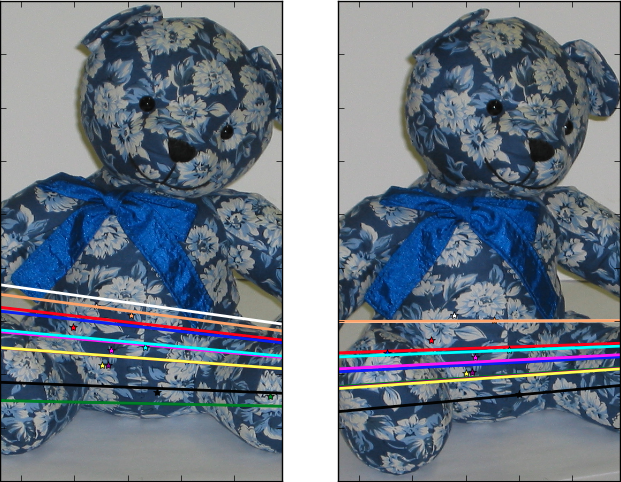
\includegraphics[width=.5\textwidth]{bear_epi}
	\caption{The epipolar constraints of two images of the teddy bear.}
	\label{fig:epipolar}
\end{figure}

The Sampson distance that is used to calculate the inliers is a approximation of the distance from a point to the epipolar lines.

We will use this to create a point view matrix, a matrix where the rows are images and columns are feature points in the images.
This matrix is of size $2m \times n$ where $m$ is the amount of cameras and $n$ the number of feature points that occur in 3 or more images. 
It is $2m \times n$ instead of $m \times n \times 2$ is so we can do Singuluar Value Decomposition.
With the results of this SVD we can create two matrices, the motion- and structure-matrices.
However as we can see in Figure~\ref{fig:pvm} not every point is seen in every image.
To deal with this we need to use a factorization method to still use Singular Value Decomposition to create a 3D point cloud that represents the teddy bear.
The factorization method that we have chosen to use is to extract dense subblocks from this point view matrix  and create multiple motion- and structure-matrices and stitch them together afterwards.

\begin{figure}[ht]
	\centering
	
\includegraphics[width=\textwidth]{pvm}
	\caption{The point view matrix of the teddy bear. Black entries represent a value, whereas a white represents a point that is not seen in that image.}
	\label{fig:pvm}
\end{figure}


\input{4_bundle.tex}
\section{Experiments}
\label{experiments}

\section{Conclusion}
\label{conclusion}


\end{document}
